\documentclass[12pt]{article}

\usepackage{sbc-template}
\usepackage{graphicx,url}
\usepackage[utf8]{inputenc}
\usepackage[brazil]{babel}
\usepackage{amsmath}
\usepackage{placeins}
\usepackage[round,authoryear,semicolon]{natbib}

% Ajuste de espaçamento de floats (recomendado SBC)
\setlength{\textfloatsep}{8pt plus 2pt minus 4pt}
\setlength{\floatsep}{8pt plus 2pt minus 4pt}
\setlength{\intextsep}{8pt plus 2pt minus 4pt}

\sloppy

\title{Arquitetura NILM \textit{Edge-to-Server} de Baixo Custo: Proposta e Avalia\c{c}\~ao N\~ao Supervisionada em Ambiente Residencial Real}

\author{
  Carlos Miguel O. M. Silva\inst{1},
}

\address{
  Instituto Federal de Mato Grosso (IFMT) \\-- Campus Cuiabá Cel. Octayde Jorge da Silva \\
  R. Zulmira Canavarros, 95 -- Centro, Cuiabá - MT, 78005-390 -- Brasil
\email{c.miguel@estudante.ifmt.edu.br}
}

\begin{document}

\maketitle

\begin{abstract}
  This paper presents the architecture of a low-cost Non-Intrusive Load
  Monitoring (NILM) system based on the Edge-to-Server paradigm. The proposed
  system distributes the processing pipeline between an embedded sensor node
  and a central server. At the edge, a hybrid architecture combining the
  STM32H743 and ESP32 microcontrollers performs high-fidelity electrical
  signal acquisition and feature extraction. Extracted features are transmitted
  via MQTT protocol for machine learning-based disaggregation on the server
  side. The approach overcomes inherent limitations of low-cost embedded
  systems -- including ADC jitter and Wi-Fi interference -- enabling accurate
  computation of active power and Total Harmonic Distortion.
  Preliminary experiments on real residential data show that unsupervised
  K-means clustering identifies appliance event signatures, but resolution
  degrades as low-power events accumulate. A permutation null test reveals that
  harmonic features, despite high-fidelity acquisition, provide no additional
  discriminative information for event-based clustering in the evaluated
  scenario. The absence of appliance labeling control during data collection
  is documented as a structural constraint of real-world NILM deployment,
  motivating future work with structured acquisition protocols.
\end{abstract}

\begin{resumo}
  Este artigo apresenta a arquitetura de um sistema de Monitoramento N\~ao
  Intrusivo de Cargas (NILM) de baixo custo relativo baseado no paradigma
  \textit{Edge-to-Server}. O sistema proposto distribui o \textit{pipeline} de
  processamento entre um n\'o sensor embarcado e um servidor central. Na borda,
  uma arquitetura h\'ibrida composta pelos microcontroladores STM32H743 e ESP32
  realiza a aquisi\c{c}\~ao de alta fidelidade e a extra\c{c}\~ao de
  caracter\'isticas dos sinais el\'etricos. As caracter\'isticas extra\'idas
  s\~ao transmitidas via protocolo MQTT para desagrega\c{c}\~ao por modelos de
  aprendizado de m\'aquina no servidor. A abordagem supera limita\c{c}\~oes
  inerentes a \textit{hardwares} embarcados de baixo custo, como \textit{jitter}
  no ADC e interfer\^encia do Wi-Fi, viabilizando o c\'alculo preciso de
  pot\^encia e Distor\c{c}\~ao Harm\^onica Total.
  Experimentos conduzidos em ambiente residencial real sem controle das cargas
  mostram que o agrupamento K-means identifica assinaturas de eventos de carga,
  mas a resolu\c{c}\~ao fina se degrada com o ac\'umulo de eventos de baixa
  pot\^encia. Um teste de nulidade por permuta\c{c}\~ao revela que as
  caracter\'isticas harm\^onicas n\~ao agregam informa\c{c}\~ao discriminativa
  ao agrupamento baseado em eventos no cen\'ario avaliado. A aus\^encia de
  controle da rotulagem durante a coleta \'e documentada como uma
  caracter\'istica estrutural do NILM em campo, direcionando trabalhos futuros
  com protocolo de aquisi\c{c}\~ao estruturado.

  \textbf{Palavras-chave:} NILM, sistemas embarcados, \textit{Edge-to-Server},
  aprendizado de m\'aquina, monitoramento n\~ao intrusivo de energia.
\end{resumo}


\section{Introdu\c{c}\~ao}

A crescente demanda por efici\^encia energ\'etica e a necessidade de redu\c{c}\~ao
do consumo de eletricidade impulsionam o desenvolvimento de tecnologias de
monitoramento inteligente \citep{ref2,ref6}. Tradicionalmente, o Monitoramento
Intrusivo de Cargas (ILM -- \textit{Intrusive Load Monitoring}) exige a
instala\c{c}\~ao de sensores dedicados para cada equipamento \citep{ref1,ref2}.
Essa abordagem resulta em altos custos e expressiva complexidade de
infraestrutura \citep{ref2,ref3}. Nesse cen\'ario, o Monitoramento N\~ao Intrusivo de
Cargas (NILM -- \textit{Non-Intrusive Load Monitoring}) configura-se como uma
alternativa vi\'avel e escal\'avel \citep{ref1,ref6}. Essa tecnologia \'e capaz de
desagregar o consumo total de uma instala\c{c}\~ao el\'etrica e estimar o consumo
individual de cada aparelho a partir de um \'unico ponto de medi\c{c}\~ao
\citep{ref1}.

Apesar dos avan\c{c}os dos algoritmos de aprendizado de m\'aquina e reconhecimento
de padr\~oes aplicados ao NILM, grande parte da literatura reporta depend\^encia
de \textit{hardware} de medi\c{c}\~ao de alto custo na borda \citep{ref6,ref7}. A
transi\c{c}\~ao parcial desses processamentos para o modelo
\textit{Edge-to-Server}, utilizando n\'os sensores baseados em sistemas embarcados
h\'ibridos de baixo custo relativo, apresenta um desafio de engenharia
significativo. Observa\c{c}\~oes emp\'iricas demonstram que as restri\c{c}\~oes
inerentes a dispositivos de recursos restritos -- tais como limita\c{c}\~oes na
taxa de amostragem, estabilidade do conversor anal\'ogico-digital (ADC) e
concorr\^encia com rotinas de comunica\c{c}\~ao Wi-Fi -- exigem uma arquitetura
cuidadosa para extra\c{c}\~ao de caracter\'isticas com alta fidelidade
\citep{ref8}.

Neste contexto, o presente artigo tem como objetivo propor e avaliar a
arquitetura de um sistema NILM \textit{Edge-to-Server} de baixo custo relativo
operando em ambiente residencial real sem controle das cargas. O trabalho
aborda dois aspectos complementares: (i)~a distribui\c{c}\~ao do
\textit{pipeline} de processamento -- extra\c{c}\~ao de caracter\'isticas na
borda (\textit{feature engineering}) e desagrega\c{c}\~ao n\~ao supervisionada
no servidor --; e (ii)~a caracteriza\c{c}\~ao dos limites dessa abordagem em
condi\c{c}\~ao real de uso, em que a rotulagem controlada \'e invi\'avel,
respondendo \`a pergunta: \textit{o que \'e poss\'ivel inferir sobre o consumo
residencial sem qualquer controle sobre as cargas ligadas?}

Este artigo est\'a organizado em sete se\c{c}\~oes, incluindo esta introdu\c{c}\~ao.
A Se\c{c}\~ao~2 apresenta o referencial te\'orico sobre NILM, seus algoritmos de
desagrega\c{c}\~ao e o paradigma \textit{Edge-to-Server}. A Se\c{c}\~ao~3 detalha
a arquitetura de \textit{hardware} e sensoriamento do sistema proposto. A
Se\c{c}\~ao~4 descreve a infraestrutura de servidor e o \textit{pipeline} de
aquisi\c{c}\~ao de dados. A Se\c{c}\~ao~5 apresenta a metodologia de
desagrega\c{c}\~ao n\~ao supervisionada adotada. A Se\c{c}\~ao~6 apresenta e
discute os resultados obtidos em ambiente residencial sem controle das cargas.
Por fim, a Se\c{c}\~ao~7 apresenta as considera\c{c}\~oes finais e os pr\'oximos
passos.


\section{Referencial Te\'orico}

\subsection{Fundamentos do Monitoramento N\~ao Intrusivo de Cargas (NILM)}

O conceito de NILM foi introduzido pioneiramente por George W. Hart no in\'icio da
d\'ecada de 1990 \citep{ref1}. O princ\'ipio elementar do m\'etodo consiste em
monitorar as formas de onda de tens\~ao e corrente no ramal de entrada de energia
(quadro de distribui\c{c}\~ao) e, mediante a an\'alise dessas medi\c{c}\~oes
agregadas, inferir as transi\c{c}\~oes de estado (ligar/desligar) e o consumo
cont\'inuo dos aparelhos conectados a jusante \citep{ref1}.

O \textit{pipeline} cl\'assico de um sistema NILM \'e estruturado em quatro etapas
fundamentais \citep{ref2,ref7}:

\begin{enumerate}
  \item \textbf{Aquisi\c{c}\~ao de Dados:} Medi\c{c}\~ao cont\'inua dos sinais
  el\'etricos. Pode ser dividida em abordagens de baixa frequ\^encia \citep{ref3}
  e alta frequ\^encia.

  \item \textbf{Detec\c{c}\~ao de Eventos:} Processo de varredura do sinal para
  identifica\c{c}\~ao de varia\c{c}\~oes bruscas que indicam a mudan\c{c}a de
  estado operacional de um equipamento \citep{ref2}.

  \item \textbf{Extra\c{c}\~ao de Caracter\'isticas (\textit{Feature
  Extraction}):} Transforma\c{c}\~ao dos sinais brutos em assinaturas el\'etricas
  \'unicas para cada equipamento \citep{ref2}. Inclui o c\'alculo de saltos de
  pot\^encia, an\'alise da trajet\'oria V-I, e quantifica\c{c}\~ao do conte\'udo
  harm\^onico mediante a Distor\c{c}\~ao Harm\^onica Total (DHT;
  $THD$ na nota\c{c}\~ao internacional) \citep{ref8}.

  \item \textbf{Classifica\c{c}\~ao e Desagrega\c{c}\~ao:} Emprego de algoritmos
  matem\'aticos ou modelos computacionais para associar as caracter\'isticas
  extra\'idas a uma classe de equipamento mapeada em um banco de dados pr\'evio
  \citep{ref4,ref6}.
\end{enumerate}

\subsection{Modelagem e Algoritmos de Desagrega\c{c}\~ao}

O n\'ucleo de intelig\^encia de um sistema NILM reside em seu algoritmo de
desagrega\c{c}\~ao. As arquiteturas de modelagem evolu\'iram de abordagens
heur\'isticas para modelos avan\c{c}ados baseados em Intelig\^encia Artificial
\citep{ref4}.

Historicamente, modelos estat\'isticos como os \textbf{Modelos Ocultos de Markov
Fatoriais (FHMM)} e t\'ecnicas de \textbf{Otimiza\c{c}\~ao Combinat\'oria}
dominaram a literatura \citep{ref2,ref3,ref4}. Com a consolida\c{c}\~ao do aprendizado de
m\'aquina, algoritmos supervisionados e baseados em dist\^ancias -- como
\textbf{K-Nearest Neighbors (KNN)}, \textbf{Support Vector Machines (SVM)} e
\textbf{Random Forests} -- ganharam espa\c{c}o devido \`a efic\'acia na
classifica\c{c}\~ao de assinaturas estacion\'arias com custo computacional moderado
\citep{ref6}.

A arquitetura do tipo sequ\^encia-para-ponto foi introduzida na literatura como um
marco estrutural para esses modelos computacionais \citep{ref5}. Nos \'ultimos anos,
t\'ecnicas de \textit{Deep Learning}, em especial \textbf{Redes Neurais
Convolucionais (CNNs)} e redes recorrentes como \textbf{Long Short-Term Memory
(LSTM)}, t\^em sido aplicadas com sucesso nessa arquitetura, definindo o estado da
arte para desagrega\c{c}\~ao \citep{ref7}. Embora altamente precisas, estas
abordagens exigem consider\'avel capacidade de processamento, o que imp\~oe uma
forte barreira para sua implementa\c{c}\~ao direta em microcontroladores de
prop\'osito geral \citep{ref7}.

\subsection{Pr\'e-processamento na Borda e Integra\c{c}\~ao Edge-to-Server}

A arquitetura \textit{Edge-to-Server} divide a carga computacional entre o n\'o
sensor (borda) e o servidor central. Em vez de executar infer\^encias pesadas no
microcontrolador, o foco na borda passa a ser a aquisi\c{c}\~ao robusta e o
pr\'e-processamento para extra\c{c}\~ao de \textit{features}, garantindo a
viabilidade de rede e de custo operacional.

\textbf{Limita\c{c}\~oes de Sensoriamento e Condicionamento:} A utiliza\c{c}\~ao
de Conversores Anal\'ogico-Digitais integrados requer metodologias rigorosas.
Testes pr\'aticos indicam que \'e necess\'ario isolar as rotinas cr\'iticas para
superar o alto \textit{jitter} de comunica\c{c}\~ao \citep{ref8}. A convers\~ao
anal\'ogico-digital (ADC) nativa em microcontroladores como o ESP32 apresenta
limita\c{c}\~oes intr\'insecas ao hardware associadas ao tempo de processamento de
aproxima\c{c}\~ao sucessiva (SAR). O microcontrolador ESP32 possui dois ADCs, por\'em
o ADC2 possui limita\c{c}\~oes de uso conjunto com o Wi-Fi, obrigando o sistema a
utilizar apenas o ADC1 para processar m\'ultiplos canais e, por consequ\^encia,
dobrando o tempo de processamento das amostras \citep{ref8}.

\textbf{Engenharia de Caracter\'isticas (\textit{Feature Engineering}):} O
microcontrolador realiza c\'alculos matem\'aticos densos localmente para evitar a
transmiss\~ao cont\'inua de ondas em alta frequ\^encia. Para assegurar precis\~ao
no c\'alculo da pot\^encia ativa e da Distor\c{c}\~ao Harm\^onica Total (DHT) por
meio da Transformada Discreta de Fourier, o ciclo de amostragem deve ser um
m\'ultiplo do per\'iodo da frequ\^encia fundamental, adotando-se de forma
recorrente um ciclo de 50ms. A placa extrai as assinaturas el\'etricas reduzindo
pacotes de megabytes para alguns kilobytes por segundo.

\textbf{Desagrega\c{c}\~ao em Servidor:} Uma vez que as \textit{features} s\~ao
transmitidas ao servidor, eliminam-se as restri\c{c}\~oes de mem\'oria RAM e de
processamento. Isso viabiliza o uso tanto de algoritmos cl\'assicos otimizados
\citep{ref6} quanto de abordagens baseadas em \textit{Deep Learning} no ambiente
servidor \citep{ref7}.

Desta forma, a viabilidade de um modelo NILM funcional em hardware de baixo custo
relativo recai sobre a qualidade e precis\~ao das abstra\c{c}\~oes de
caracter\'isticas el\'etricas na borda.


\section{Arquitetura do Sistema Proposto}

Motivado por esse contexto, esta se\c{c}\~ao detalha as decis\~oes de engenharia e
a arquitetura adotada para a concep\c{c}\~ao do medidor inteligente. O projeto foi
guiado pela necessidade de conciliar a extra\c{c}\~ao de m\'etricas el\'etricas de
alta fidelidade com as restri\c{c}\~oes de processamento, mem\'oria e custo de
sistemas embarcados comerciais.

\subsection{Arquitetura Edge-to-Server}

O sistema foi concebido sob o paradigma \textit{Edge-to-Server}, onde a aquisi\c{c}\~ao
prim\'aria e o pr\'e-processamento ocorrem localmente, enquanto os dados s\~ao
transmitidos para um servidor para desdobramento do modelo NILM. Essa abordagem
otimiza o uso da rede. O fluxo de dados passa pelos est\'agios de sensoriamento,
condicionamento, processamento embarcado e comunica\c{c}\~ao.

\subsection{Arquitetura de Hardware e Sensoriamento}

Para garantir um monitoramento n\~ao intrusivo, optou-se pela utiliza\c{c}\~ao de
sensores que n\~ao requerem seccionamento da fia\c{c}\~ao original.

\subsubsection{Sensoriamento de Corrente e Tens\~ao}

A medi\c{c}\~ao de corrente \'e realizada pelo Transformador de Corrente (TC)
\textbf{SCT-013}, do tipo n\'ucleo dividido. Para a medi\c{c}\~ao de tens\~ao,
adotou-se o transformador de potencial isolador \textbf{ZMPT101B}. Devido a
limita\c{c}\~oes f\'isicas inerentes aos transdutores, os sinais condicionados
apresentam defasagem em rela\c{c}\~ao aos sinais originais e tamb\'em entre si.
Para executar c\'alculos realistas da pot\^encia e fator de pot\^encia, \'e imperativo
corrigir tal defasagem deslocando o vetor completo do sinal da corrente por uma
quantidade calculada de amostras em rela\c{c}\~ao ao vetor de tens\~ao.

Durante a fase de valida\c{c}\~ao, identificou-se que os m\'odulos comerciais
baseados no ZMPT101B introduziam distor\c{c}\~oes harm\^onicas indesejadas e
causavam defasagem angular no sinal medido. Como solu\c{c}\~ao, optou-se por
utilizar o componente ZMPT101B isolado (\textit{standalone}), implementando-se um
circuito condicionador passivo e customizado.

\subsubsection{Processamento H\'ibrido com STM32H743 e ESP32}

A concep\c{c}\~ao inicial previa a utiliza\c{c}\~ao exclusiva do microcontrolador
ESP32 para amostragem (via ADC nativo) e comunica\c{c}\~ao. Entretanto, as
interrup\c{c}\~oes geradas pelo \textit{stack} de comunica\c{c}\~ao Wi-Fi no ESP32
causavam varia\c{c}\~oes temporais (\textit{jitter}) severas na amostragem.

A an\'alise das capacidades do ESP32 demonstra que o temporizador de alta
resolu\c{c}\~ao (\textit{High-Resolution Timer} -- HRT) pode possuir um per\'iodo
m\'inimo de $50\,\mu\text{s}$ (te\'oricos 20\,kHz), mas em aplica\c{c}\~oes de mundo
real a tentativa de utilizar taxas t\~ao altas aciona o temporizador vigia
(\textit{watchdog timer}) do sistema \citep{ref8}. Nos ensaios experimentais, a
amostragem de um \'unico canal estabilizou-se na marca de $80\,\mu\text{s}$. Como o
projeto exigiu a medi\c{c}\~ao paralela de dois canais alocados apenas no ADC1,
estabeleceu-se a taxa de amostragem vi\'avel em $200\,\mu\text{s}$ (5\,kHz) para
garantir a estabilidade. Embora o ciclo de 5\,kHz permita a obten\c{c}\~ao de 250
amostras por canal em 50\,ms (suficiente para o c\'alculo at\'e a 41\textordfeminine~harm\^onica),
o compartilhamento de processamento com o m\'odulo de r\'adio permanecia como um
gargalo estrutural \citep{ref8}.

Para superar esse desafio, a arquitetura foi redesenhada para um modelo h\'ibrido:

\begin{enumerate}
  \item \textbf{STM32H743 (Processamento de Sinal):} Selecionado pelo seu ADC de
  alta resolu\c{c}\~ao e capacidade superior de \textit{Digital Signal Processing}
  (DSP). Este microcontrolador atua dedicado exclusivamente \`a aquisi\c{c}\~ao
  ininterrupta e de alta fidelidade das formas de onda de tens\~ao e corrente,
  realizando o c\'alculo local das grandezas el\'etricas.

  \item \textbf{ESP32 (Comunica\c{c}\~ao):} Atua como m\'odulo de conectividade
  Wi-Fi e gerenciador de pacotes. O dispositivo assume exclusivamente a
  integra\c{c}\~ao de rede, transmitindo os indicadores como pot\^encia ativa e
  DHT consolidados para a infraestrutura via protocolo MQTT
  (\textit{Message Queuing Telemetry Transport}).
\end{enumerate}

O fluxo de dados entre o STM32H743 e o ESP32 \'e realizado via barramento serial
UART (\textit{Universal Asynchronous Receiver-Transmitter}). Como as rotinas de
amostragem pesadas foram transferidas para o STM32 e apenas as vari\'aveis
calculadas s\~ao transmitidas ao ESP32, a largura de banda da comunica\c{c}\~ao
serial mostrou-se perfeitamente adequada.


\section{Infraestrutura de Servidor e \textit{Pipeline} de Aquisi\c{c}\~ao}

Com o n\'o de borda configurado conforme descrito na se\c{c}\~ao anterior, a camada
de servidor materializa a por\c{c}\~ao \textit{server} do paradigma
\textit{Edge-to-Server}. O n\'o ESP32 publica as caracter\'isticas calculadas
via protocolo MQTT em um \textit{broker} Mosquitto hospedado em um servidor
dedicado, fisicamente distinto da esta\c{c}\~ao de desenvolvimento. Essa
separa\c{c}\~ao garante que a aquisi\c{c}\~ao permane\c{c}a cont\'inua e
independente do ambiente de an\'alise.

A comunica\c{c}\~ao \'e organizada em dois t\'opicos: \texttt{energia/medidor},
que transporta as grandezas el\'etricas consolidadas por ciclo, e
\texttt{energia/harmonicas}, que transporta o espectro harm\^onico. Um processo
assinante (\textit{ingestor}) persiste cada mensagem em arquivos CSV
(\textit{Comma-Separated Values}) sequenciais, formando a base de dados de
treinamento. Tanto o \textit{broker} quanto o \textit{ingestor} s\~ao executados como
servi\c{c}os resilientes, com in\'icio autom\'atico na inicializa\c{c}\~ao do sistema
e rein\'icio autom\'atico em caso de falha, assegurando registro ininterrupto.

Cada mensagem de medi\c{c}\~ao agrega, por fase: tens\~ao e corrente eficazes
($V_{rms}$, $I_{rms}$), pot\^encia ativa ($P$), pot\^encia reativa ($Q$),
pot\^encia aparente ($S$), fator de pot\^encia (FP) e energia acumulada (kWh).
As mensagens harm\^onicas carregam a Distor\c{c}\~ao Harm\^onica Total de tens\~ao
e corrente ($THD_V$ e $THD_I$, conforme nota\c{c}\~ao definida na Se\c{c}\~ao~2) e
a magnitude das 50 primeiras componentes harm\^onicas de tens\~ao e de corrente.

\begin{figure}[ht]
  \centering
  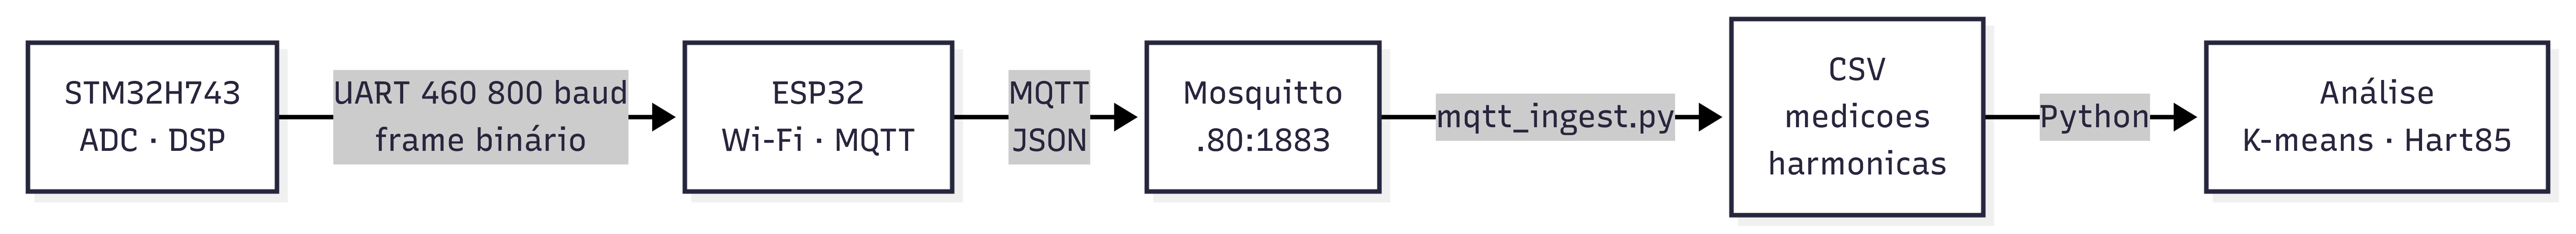
\includegraphics[width=\linewidth]{figuras/fluxo-de-dados.png}
  \caption{Fluxo de dados da arquitetura \textit{Edge-to-Server}.}
  \label{fig:pipeline}
\end{figure}


\section{Metodologia de Desagrega\c{c}\~ao por Aprendizado de M\'aquina}

De posse das caracter\'isticas adquiridas e persistidas conforme descrito na
se\c{c}\~ao anterior, a desagrega\c{c}\~ao no servidor segue uma abordagem
orientada a eventos combinada com aprendizado n\~ao supervisionado, adequada a
cen\'arios reais em que n\~ao h\'a controle expl\'icito sobre as cargas
conectadas.

\subsection{Conjunto de Caracter\'isticas}

O vetor de caracter\'isticas associado a cada evento \'e composto pelas
varia\c{c}\~oes das grandezas de regime permanente -- com destaque para os
saltos de pot\^encia ativa ($\Delta P$) e reativa ($\Delta Q$) -- e,
opcionalmente, pelo conte\'udo harm\^onico ($THD_V$, $THD_I$ e harm\^onicas
dominantes). A disponibilidade do espectro harm\^onico pode, em tese,
fornecer uma assinatura adicional discriminativa para cargas n\~ao lineares,
cujo perfil difere de cargas resistivas (pr\'oximas da senoidal);
sua contribui\c{c}\~ao efetiva \'e avaliada empiricamente na Se\c{c}\~ao~6.

\subsection{Detec\c{c}\~ao de Eventos}

A detec\c{c}\~ao de eventos emprega o princ\'ipio cl\'assico de Hart \citep{ref1}:
uma linha de base m\'ovel acompanha o regime permanente, e uma transi\c{c}\~ao
\'e registrada quando a pot\^encia ativa apresenta um degrau superior a um limiar
configur\'avel, sustentado por um n\'umero m\'inimo de amostras consecutivas. O
processamento \'e realizado de forma independente por fase. Cargas que n\~ao
produzem degraus discretos -- discutidas na Se\c{c}\~ao de resultados -- s\~ao
tratadas de forma complementar.

\subsection{Agrupamento N\~ao Supervisionado de Assinaturas}

Os eventos detectados s\~ao agrupados por meio do algoritmo \textbf{K-means} no
espa\c{c}o de caracter\'isticas. O n\'umero de \textit{clusters} $K$ \'e
selecionado automaticamente pelo coeficiente de \textbf{silhueta}, que quantifica
a coes\~ao interna e a separa\c{c}\~ao entre grupos sem necessidade de
r\'otulos pr\'evios. Cada \textit{cluster} corresponde a uma assinatura
el\'etrica recorrente, candidata a um aparelho ou estado operacional.

\subsection{Interpretação dos Agrupamentos e Limites do Ambiente N\~ao Controlado}

Em ambientes residenciais reais, a coleta raramente pode ser realizada com
controle total sobre o que foi ligado e quando. Neste trabalho, a coleta foi
conduzida de forma cont\'inua e passiva: n\~ao houve protocolo de acionamento
controlado, de modo que a associa\c{c}\~ao iqu\'ivoca entre um evento el\'etrico
detectado e um aparelho espec\'ifico \'e, em grande parte dos casos, imposs\'ivel.
Essa condi\c{c}\~ao -- denominada aus\^encia de \textit{ground truth} -- torna a
classifica\c{c}\~ao supervisionada cl\'assica impratic\'avel sem comprometer a
integridade dos resultados.

A abordagem adotada \'e, portanto, integralmente n\~ao supervisionada. Os
\textit{clusters} formados pelo K-means s\~ao interpretados \textit{a posteriori}
quanto \`a plausibilidade f\'isica: magnitude de $\Delta P$, sinal de $\Delta Q$
e assinatura harm\^onica. Um \textit{cluster} \'e associado a uma categoria de
equipamento apenas quando a evid\^encia \'e suficientemente discriminativa -- por
exemplo, um grupo isolado com $\Delta P \approx +2{,}3$~kW e elevado $\Delta Q$
\'e consistente com um compressor de ciclo de compress\~ao. Grupos amb\'iguos
permanecem como categoria ``desconhecida''.

Essa limita\c{c}\~ao n\~ao \'e uma falha do m\'etodo, mas uma propriedade
documentada do NILM em campo: a necessidade de controle da coleta para viabilizar
a classifica\c{c}\~ao supervisionada \'e, ela pr\'opria, um resultado deste
trabalho. As impress\~oes sobre quais aparelhos foram identificados s\~ao
discutidas na an\'alise de erro (Se\c{c}\~ao~6.3) e motivam o delineamento do
protocolo de coleta estruturado proposto como trabalho futuro.

\subsection{Estudo de Abla\c{c}\~ao}

Para mensurar a contribui\c{c}\~ao das caracter\'isticas harm\^onicas, aplica-se
um \textbf{teste de nulidade por permuta\c{c}\~ao}: a qualidade do agrupamento
(coeficiente de silhueta) obtida com as caracter\'isticas harm\^onicas reais \'e
comparada \`a obtida com essas mesmas caracter\'isticas \textbf{embaralhadas} --
quebrando o v\'inculo evento--harm\^onico. Se a estrutura harm\^onica fosse
discriminativa, a silhueta com dados reais deveria superar a embaralhada de forma
consistente. O teste \'e aplicado separadamente a dois conjuntos de
\textit{features}: (i)~apenas pot\^encias ($\Delta P$, $\Delta Q$) como linha de
base; (ii)~pot\^encias acrescidas do conte\'udo harm\^onico, tanto em termos
absolutos (THD e harm\^onicas no instante do evento) quanto em varia\c{c}\~ao
($\Delta$harm\^onico, p\'os menos pr\'e-evento). A diferen\c{c}a de silhueta entre
real e embaralhado quantifica o ganho real proporcionado pela aquisi\c{c}\~ao de
alta fidelidade na borda.


\section{Resultados e Discuss\~ao}

Esta se\c{c}\~ao apresenta os resultados obtidos a partir de coleta cont\'inua e
passiva em ambiente residencial real sem controle das cargas. A aus\^encia de
protocolo estruturado de acionamento -- condi\c{c}\~ao deliberada para avaliar o
comportamento do sistema em uso cotidiano -- imp\~oe o emprego exclusivo de
m\'etodos n\~ao supervisionados e m\'etricas internas de qualidade (silhueta,
estabilidade dos agrupamentos e plausibilidade f\'isica).

\subsection{Evolu\c{c}\~ao Temporal e Dilui\c{c}\~ao por Cargas de Baixa
Pot\^encia}

Para avaliar a robustez da descoberta n\~ao supervisionada, o agrupamento sobre
($\Delta P$, $\Delta Q$) foi repetido em janelas de coleta crescentes (de 12 a
48~horas; limiar de detec\c{c}\~ao de 50~W). A Figura~\ref{fig:clusters1d2d}
contrasta os dois extremos.

Com \textbf{um dia} de coleta (727 eventos), o K-means resolve $K=10$
\textit{clusters} aparentes, com diversos aparelhos de pot\^encia m\'edia surgindo
como grupos distintos. Contudo, o coeficiente de silhueta correspondente \'e baixo
(0{,}44), indicando \textbf{sobre-segmenta\c{c}\~ao}: a estrutura fina n\~ao \'e
estatisticamente robusta. Com \textbf{dois dias} (1270 eventos), o $K$ \'otimo
\textbf{colapsa para 3} (silhueta 0{,}74): um \'unico \textit{cluster} dominante de
eventos de baixa pot\^encia, somado aos dois extremos -- o motor de
$\approx$2{,}3~kW (alto $\Delta Q$) e as cargas resistivas de alta pot\^encia. Os
grupos de pot\^encia m\'edia, separ\'aveis em um dia, foram \textbf{absorvidos}
pela massa de baixa pot\^encia.

\begin{figure}[ht]
  \centering
  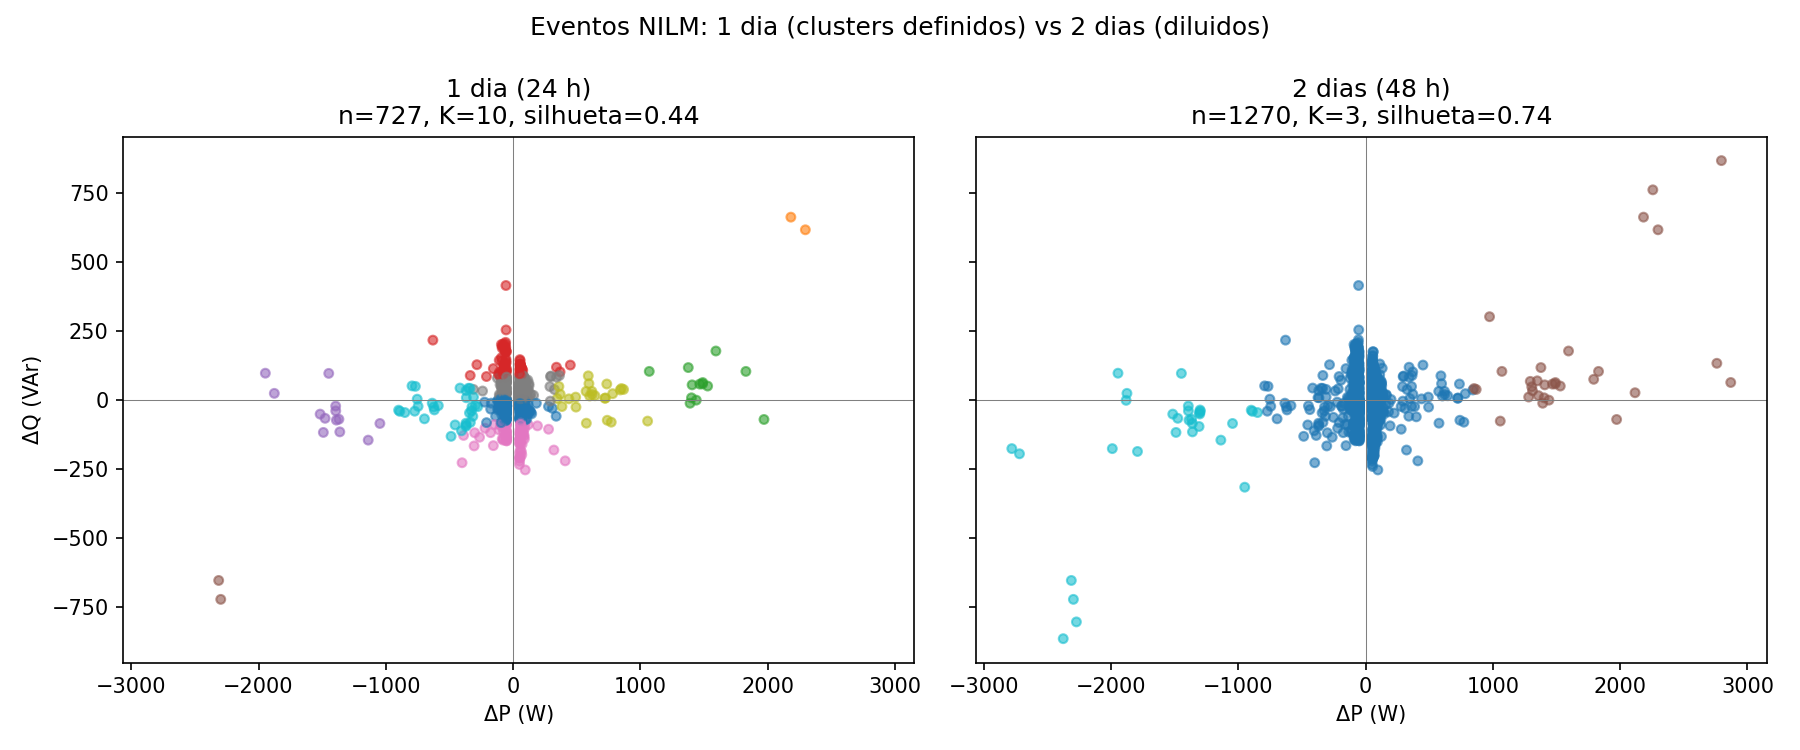
\includegraphics[width=\linewidth]{figuras/clusters_1d2d.png}
  \caption{Eventos no plano $\Delta P \times \Delta Q$. Com um dia (esquerda) o
  K-means resolve dez grupos (silhueta 0{,}44, sobre-segmenta\c{c}\~ao); com dois
  dias (direita) a massa de baixa pot\^encia domina e o agrupamento colapsa para
  tr\^es (silhueta 0{,}74).}
  \label{fig:clusters1d2d}
\end{figure}

O mecanismo \'e a \textbf{dilui\c{c}\~ao por cargas de baixa pot\^encia}. Cerca de
85\% de todos os eventos s\~ao degraus de baixa pot\^encia ($|\Delta P| < 150$~W)
originados de cargas continuamente vari\'aveis (o compressor \textit{inverter}) e
do ru\'ido de medi\c{c}\~ao. Conforme a coleta avan\c{c}a, esses eventos se
acumulam (de 361 para 1101 -- Figura~\ref{fig:degradacao}) e a qualidade da
resolu\c{c}\~ao fina (silhueta com $K$ fixo em 8) decai de 0{,}46 para 0{,}41. A
massa de baixa pot\^encia cresce at\'e dominar o espa\c{c}o de caracter\'isticas, e
o crit\'erio de silhueta passa a favorecer o agrupamento grosseiro.

\begin{figure}[ht]
  \centering
  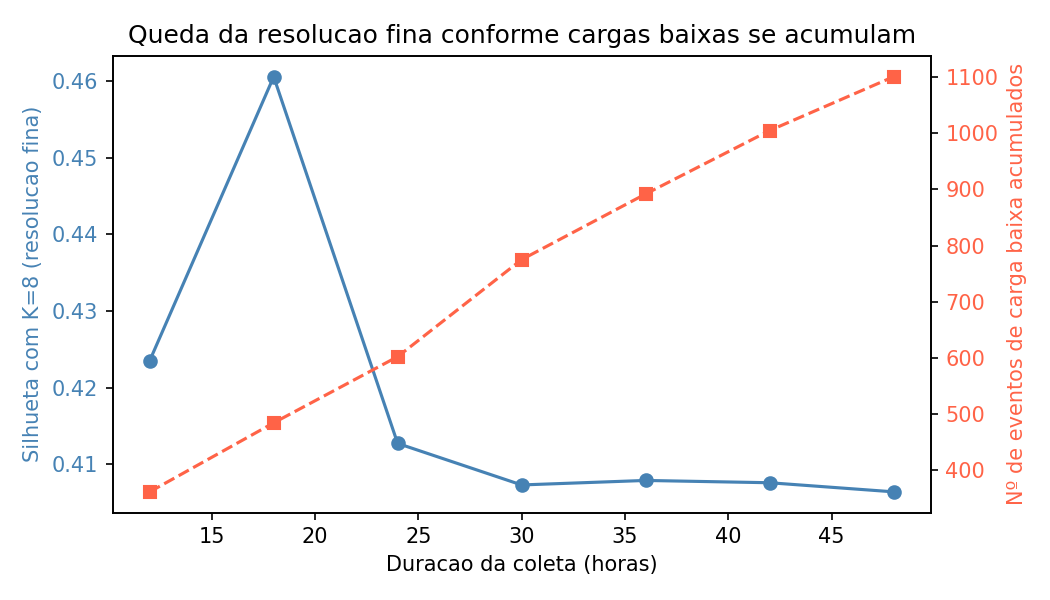
\includegraphics[width=0.8\linewidth]{figuras/degradacao.png}
  \caption{Degrada\c{c}\~ao da resolu\c{c}\~ao fina (silhueta com $K=8$, eixo
  esquerdo) conforme os eventos de baixa pot\^encia se acumulam (eixo direito) ao
  longo da coleta.}
  \label{fig:degradacao}
\end{figure}

Conclui-se que a aparente riqueza de aparelhos observada com um dia de dados
\textbf{n\~ao \'e robusta}: trata-se de sobre-segmenta\c{c}\~ao de um espa\c{c}o de
caracter\'isticas de baixa rela\c{c}\~ao sinal-ru\'ido, dominado por eventos de
baixa pot\^encia n\~ao resol\'uveis. Apenas as cargas de maior pot\^encia
permanecem separ\'aveis de forma est\'avel -- limita\c{c}\~ao consistente com as
restri\c{c}\~oes de sensoriamento (n\~ao-linearidade do SCT-013 em baixa corrente
e erro de fase dos transdutores) discutidas a seguir.

\subsection{Avalia\c{c}\~ao das Caracter\'isticas Harm\^onicas}

A aquisi\c{c}\~ao harm\^onica de alta fidelidade \'e um diferencial da arquitetura
na borda; sua contribui\c{c}\~ao para a desagrega\c{c}\~ao, por\'em, foi avaliada de
forma rigorosa, e o resultado \'e nulo neste cen\'ario -- o que constitui, em si,
um achado relevante.

Aplicou-se um \textbf{teste de nulidade} por permuta\c{c}\~ao: compara-se a silhueta
do agrupamento com as caracter\'isticas harm\^onicas reais contra a mesma
clusteriza\c{c}\~ao com essas caracter\'isticas \textbf{embaralhadas} (quebrando o
v\'inculo evento--harm\^onico). Se a estrutura fosse real, a silhueta com dados
reais superaria a embaralhada. Para o conte\'udo harm\^onico \textbf{absoluto}
(THD e harm\^onicas no instante do evento), a silhueta real (0{,}194) foi
praticamente id\^entica \`a embaralhada (0{,}191) -- ambas muito acima de dados
puramente aleat\'orios (0{,}051). Ou seja, existe estrutura, mas ela prov\'em de
$\Delta P$/$\Delta Q$, n\~ao dos harm\^onicos.

A an\'alise foi refeita com a \textbf{varia\c{c}\~ao} harm\^onica
($\Delta$harm\^onico, p\'os menos pr\'e-evento, an\'aloga a $\Delta P$), que isola a
assinatura do aparelho chaveado. Como mostra a Figura~\ref{fig:ablacao}, acrescentar
o $\Delta$harm\^onico \`as pot\^encias n\~ao apenas falha em melhorar, como
\textbf{degrada} a silhueta (de 0{,}43 para 0{,}14); e o valor real (0{,}139)
novamente coincide com o embaralhado (0{,}122).

\begin{figure}[ht]
  \centering
  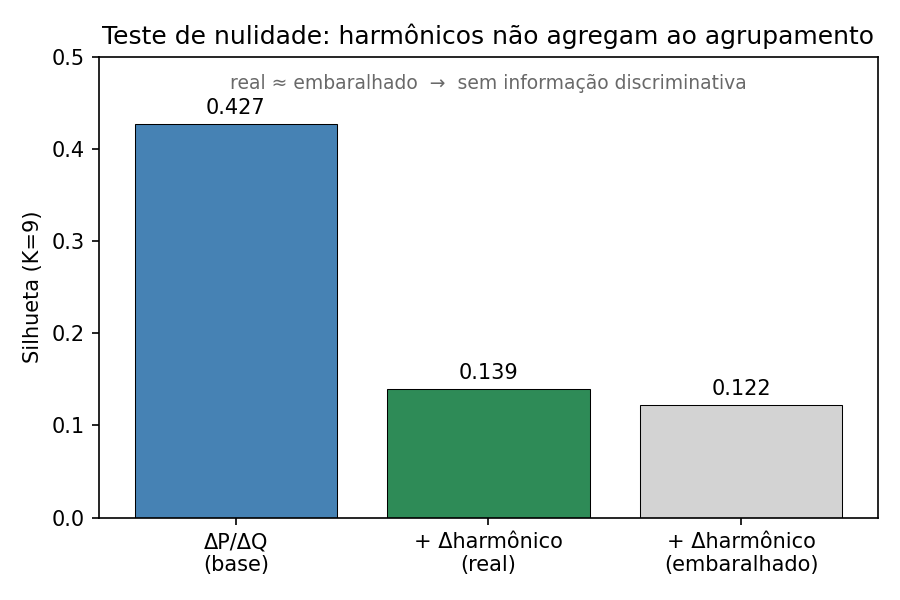
\includegraphics[width=0.7\linewidth]{figuras/ablacao_harmonicos.png}
  \caption{Teste de nulidade das caracter\'isticas harm\^onicas. A silhueta com
  $\Delta$harm\^onico real \'e estatisticamente igual \`a obtida com os mesmos
  valores embaralhados, e inferior \`a base $\Delta P$/$\Delta Q$ -- evid\^encia de
  que os harm\^onicos n\~ao agregam informa\c{c}\~ao discriminativa ao agrupamento.}
  \label{fig:ablacao}
\end{figure}

Conclui-se que, neste \textit{setup}, os harm\^onicos -- absolutos ou em
varia\c{c}\~ao -- n\~ao carregam informa\c{c}\~ao \'util ao agrupamento de eventos.
As causas prov\'aveis s\~ao: (i)~o n\'ivel harm\^onico absoluto \'e dominado pela
assinatura de fundo da resid\^encia (cargas sempre-ligadas), e n\~ao pela carga que
chaveou; (ii)~a maioria dos eventos \'e de baixa pot\^encia, pr\'oxima ao piso de
ru\'ido, onde a medi\c{c}\~ao harm\^onica \'e pouco confi\'avel; e
(iii)~limita\c{c}\~oes de sensoriamento -- a resposta em alta frequ\^encia do
SCT-013 e a distor\c{c}\~ao residual do condicionamento de tens\~ao podem fazer o
harm\^onico medido refletir mais o sensor do que a carga. O achado n\~ao invalida o
uso de harm\^onicos em NILM, mas indica que sua explora\c{c}\~ao exigiria
sele\c{c}\~ao supervisionada de caracter\'isticas e/ou melhoria do condicionamento
-- direcionamentos para trabalho futuro.

\subsection{Desafios e An\'alise de Erro}

A coleta em ambiente n\~ao controlado introduz fontes de erro que constituem, por
si s\'o, um resultado relevante e s\~ao discutidas a seguir.

\textbf{Cargas continuamente vari\'aveis.} Aparelhos com acionamento por
\textit{inversor de frequ\^encia} -- como refrigeradores modernos -- n\~ao
desligam o compressor, mas modulam continuamente sua velocidade. Tais cargas
correspondem ao Tipo~IV da taxonomia de Hart e da literatura moderna \citep{ref1,ref7} e n\~ao
produzem degraus discretos de liga/desliga, n\~ao sendo capturadas pela detec\c{c}\~ao
de eventos convencional. Sua identifica\c{c}\~ao depende da assinatura de regime
permanente e, sobretudo, do perfil harm\^onico do est\'agio retificador do
inversor -- o que refor\c{c}a a relev\^ancia da aquisi\c{c}\~ao harm\^onica na
borda.

\textbf{Natureza da pot\^encia reativa.} A pot\^encia reativa \'e calculada na
borda como $Q = \sqrt{S^2 - P^2}$, isto \'e, como magnitude n\~ao sinalizada. O
sinal observado decorre exclusivamente de conven\c{c}\~ao de medi\c{c}\~ao
(orienta\c{c}\~ao do transformador de corrente) e n\~ao distingue cargas
indutivas de capacitivas; adota-se, portanto, o valor absoluto $|Q|$ como
caracter\'istica.

\textbf{Rotulagem incerta.} Sem controle das cargas, parte das assinaturas n\~ao
pode ser atribu\'ida a um aparelho com certeza. Casos de rotulagem incorreta s\~ao
documentados e atribu\'idos a causas espec\'ificas -- sobreposi\c{c}\~ao de
assinaturas de pot\^encia semelhante, eventos simult\^aneos somados em um \'unico
degrau, presen\c{c}a de cargas cont\'inuas e ru\'ido de medi\c{c}\~ao --,
constituindo a an\'alise de erro do trabalho. A valida\c{c}\~ao recorre a
m\'etricas internas (silhueta, estabilidade dos \textit{clusters} e
plausibilidade f\'isica) na aus\^encia de \textit{ground truth} completo.


\section{Considera\c{c}\~oes Finais}

Este artigo propôs, descreveu e avaliou a arquitetura de um sistema NILM
constru\'ido sob o paradigma \textit{Edge-to-Server}, operando em ambiente
residencial real sem controle das cargas. O trabalho respondeu \`a pergunta
central do projeto: \textit{o que \'e poss\'ivel inferir sobre o consumo
residencial sem qualquer controle sobre as cargas ligadas?}

A resposta tem duas dimens\~oes. No plano da engenharia, demonstrou-se que a
extra\c{c}\~ao de caracter\'isticas el\'etricas de alta fidelidade em
\textit{hardware} de baixo custo requer decis\~oes criteriosas: a ado\c{c}\~ao
do ZMPT101B em modo \textit{standalone} eliminou n\~ao-linearidades de
condicionamento, e a arquitetura h\'ibrida STM32H743 + ESP32 resolveu o
conflito entre amostragem de alta velocidade e comunica\c{c}\~ao Wi-Fi
\citep{ref8}, viabilizando o c\'alculo ininterrupto da pot\^encia e da DHT
sem \textit{jitter}.

No plano do aprendizado de m\'aquina, tr\^es resultados respondem \`a pergunta
central. Primeiro, a clusteriza\c{c}\~ao K-means \'e capaz de discriminar
assinaturas em janelas curtas (silhueta de 0{,}46 com um dia), mas a
resolu\c{c}\~ao fina colapsa conforme eventos de baixa pot\^encia se acumulam:
com dois dias, o $K$ \'otimo cai de dez para tr\^es, e apenas as cargas de maior
pot\^encia permanecem separ\'aveis de forma est\'avel. Segundo, o teste de
nulidade por permuta\c{c}\~ao demonstrou que as caracter\'isticas harm\^onicas
n\~ao agregam informa\c{c}\~ao discriminativa neste cen\'ario, mesmo com aquisi\c{c}\~ao
de alta fidelidade na borda -- achado que aponta para limites do sensoriamento e
n\~ao apenas do algoritmo. Terceiro, e mais importante para o contexto da
mat\'eria, a aus\^encia de controle das cargas durante a coleta revelou-se uma
barreira estrutural para a classifica\c{c}\~ao supervisionada: sem
\textit{ground truth} confi\'avel, m\'etricas como F1-macro n\~ao podem ser
calculadas sem risco de invalida\c{c}\~ao dos resultados.

Como trabalhos futuros, o passo mais imediato e estruturante \'e a realiza\c{c}\~ao
de uma campanha de coleta com protocolo controlado: acionar cada aparelho
individualmente, registrar os instantes de liga/desliga e construir um
\textit{dataset} com rotulagem confi\'avel. Isso viabilizar\'a a avalia\c{c}\~ao
de classificadores supervisionados (KNN, SVM, \textit{Random Forest}) com
m\'etricas objetivas por classe, completando o ciclo do sistema inteligente
proposto. Complementarmente, investigar estrat\'egias de filtragem dos eventos de
baixa pot\^encia -- principal fator de degrada\c{c}\~ao identificado -- e melhorias
no condicionamento harm\^onico, cujos limites foram caracterizados pelo teste de
nulidade.


% -----------------------------------------------------------------------
% DECLARAÇÃO DE IA GENERATIVA (obrigatória pela política SBC, se aplicável)
% Descomente e preencha se ferramentas de IA foram utilizadas na redação.
% -----------------------------------------------------------------------
% \section*{Declara\c{c}\~ao de Uso de Intelig\^encia Artificial Generativa}
% Este artigo utilizou a ferramenta Claude Opus 4.8 (Anthropic) como
% aux\'ilio na revis\~ao textual e estrutura\c{c}\~ao do artigo.
% Todo o conte\'udo foi verificado, validado e \'e de inteira responsabilidade
% dos autores.

\begin{thebibliography}{99}

\bibitem[Hart(1992)]{ref1} HART, G. W. Nonintrusive appliance load monitoring.
  \textit{Proceedings of the IEEE}, v.~80, n.~12, p.~1870--1891, 1992.

\bibitem[Zoha et al.(2012)]{ref2} ZOHA, A. et al. Non-Intrusive Load Monitoring Approaches for
  Disaggregated Energy Sensing: A Survey. \textit{Sensors}, v.~12,
  p.~16838--16866, 2012.

\bibitem[Chatterjee e Heer(2025)]{ref3} CHATTERJEE, A.; HEER, P. Non-Intrusive Load Monitoring (NILM)
  with very low-frequency data from smart meters in Switzerland.
  \textit{Energy and Buildings}, v. 344, 116002, 2025.

\bibitem[Kalinke et al.(2021)]{ref4} KALINKE, F. et al. An Evaluation of NILM Approaches on
  Industrial Energy-Consumption Data. In: \textit{The Twelfth ACM
  International Conference on Future Energy Systems (e-Energy '21)}, 2021.

\bibitem[Zhang et al.(2018)]{ref5} ZHANG, C. et al. Sequence-to-point learning with neural
  networks for non-intrusive load monitoring. In: \textit{AAAI Conference on
  Artificial Intelligence}, 2018.

\bibitem[Garcia et al.(2020)]{ref6} GARCIA, F. D. et al. NILM-based approach for energy efficiency
  assessment of household appliances. \textit{Energy Informatics}, v.~3,
  n.~10, 2020.

\bibitem[Nourollahi et al.(2024)]{ref7} NOUROLLAHI, H. et al. Non-Intrusive Load Monitoring using
  Machine Learning and Deep Learning Techniques. \textit{Electronics}, v.~13,
  n.~1420, 2024.

\bibitem[Resende et al.(2022)]{ref8} RESENDE, R. A. O.; PESTANA NETO, A.; RAMOS, J. J. G.
  Caracter\'isticas da convers\~ao anal\'ogico-digital (ADC -- Analog to
  Digital Conversion) nativa do microcontrolador ESP32: uma discuss\~ao. In:
  \textit{Semin\'ario em Tecnologia da Informa\c{c}\~ao do Programa de
  Capacita\c{c}\~ao Institucional (PCI) do CTI Renato Archer XII}, 2022.

\end{thebibliography}

\end{document}